%% -*- latex -*-
%%%%%%%%%%%%%%%%%%%%%%%%%%%%%%%%%%%%%%%%%%%%%%%%%%%%%%%%%%%%%%%%
%%%%
%%%% This TeX file is part of the course
%%%% Introduction to Scientific Programming in C++/Fortran2003
%%%% copyright 2018-2021 Victor Eijkhout eijkhout@tacc.utexas.edu
%%%%
%%%% gerry.tex : exercises about redistricting
%%%%
%%%%%%%%%%%%%%%%%%%%%%%%%%%%%%%%%%%%%%%%%%%%%%%%%%%%%%%%%%%%%%%%

In this project you can explore `gerrymandering', the strategic drawing
of districts to give a minority population a majority of
districts\footnote{This project is obviously based on the Northern
  American political system. Hopefully the explanations here are clear
  enough. Please contact the author if you know of other countries
  that have a similar system.}.

\Level 0 {Basic concepts}

We are dealing with the following concepts:
\begin{itemize}
\item A state is divided into census districts, which are given. Based
  on census data (income, ethnicity, median age) one can
  usually make a good guess as to the overall voting in such a
  district. 
\item There is a predetermined number of congressional districts, each
  of which 
  consists of census districts. A~congressional district is not a
  random collection: the census districts have to be contiguous.
\item Every couple of years, to account for changing populations, the
  district boundaries are redrawn. This is known as redistricting.
\end{itemize}
There is considerable freedom in how redistricting is done: by shifting the
boundaries of the (congressional) districts it is possible to give a
population that is in the overall minority a majority of districts. This is
known as \indexterm{gerrymandering}.

For background reading, see \url{https://redistrictingonline.org/}.

To do a small-scale computer simulation of gerrymandering, we make
some simplifying assumption.
\begin{itemize}
\item First of all, we dispense with census district: we assume that a
  district consists directly of voters, and that we know their
  affiliation. In practice one relies on proxy measures (such as
  income and education level) to predict affiliation.
\item Next, we assume a one-dimensional state. This is enough to
  construct examples that bring out the essence of the problem:
\begin{quotation}
  \noindent
  Consider a state of five voters, and we designate their votes as
  \n{AAABB}. Assigning them to three (contiguous) districts can be
  done as \n{AAA|B|B}, which has one `A'~district and two
  `B'~districts.
\end{quotation}
\item We also allow districts to be any positive size, as long as the
  number of districts is fixed.
\end{itemize}

\Level 0 {Basic functions}

\Level 1 {Voters}

We dispense with census districts, expressing everything in terms of
voters, for which we assume a known voting behaviour. Hence, we need a
\n{Voter} class, which will record the voter ID and party
affiliation. We assume two parties, and leave an option for being undecided.

\begin{exercise}
  Implement a \n{Voter} class. You could for instance let $\pm1$ stand
  for \n{A/B}, and 0 for undecided.
  %
  \verbatimsnippet{voterpos}
  \verbatimsnippet{voterneg}
  \verbatimsnippet{voterwrong}
\end{exercise}

\Level 1 {Populations}

\begin{exercise}
  Implement a \n{District} class that models a group of voters.
  \begin{itemize}
    \item You probably want to create a district out of a single
      voter, or a vector of them. Having a constructor that accepts a
      string representation would be nice too.
    \item Write methods \n{majority} to give the exact majority or
      minority, and \n{lean} that evaluates whether the district
      overall counts as A~part or B~party.
    \item Write a \n{sub} method to creates subsets.
\begin{lstlisting}
District District::sub(int first,int last);
\end{lstlisting}
  \item For debugging and reporting it may be a good idea to have a method
\begin{lstlisting}
string District::print();
\end{lstlisting}
  \end{itemize}
  \answerwithoutput{district}{gerry}{district}
\end{exercise}

\begin{exercise}
  Implement a \n{Population} class that will initially model a whole state.
  %
  \answerwithoutput{populationexample}{gerry}{population}

  In addition to an explicit creation, also write a constructor that
  specifies how many people and what the majority is:
  %
  \verbatimsnippet{randompopulation}
  %
  Use a random number generator to achieve precisely the indicated majority.
\end{exercise}

\Level 1 {Districting}

The next level of complication is to have a set of districts.
Since we
will be creating this incrementally, we need some methods for
extending it.

\begin{exercise}
  Write a class \n{Districting} that stores a \n{vector} of
  \n{District} objects. Write \n{size} and \n{lean} methods:
  %
  \answerwithoutput{gerryempty}{gerry}{gerryempty}
\end{exercise}

\begin{exercise}
  Write methods to extend a \n{Districting}:
  %
  \verbatimsnippet{gerryextend}
\end{exercise}

\Level 0 {Strategy}

\begin{figure}[ht]
  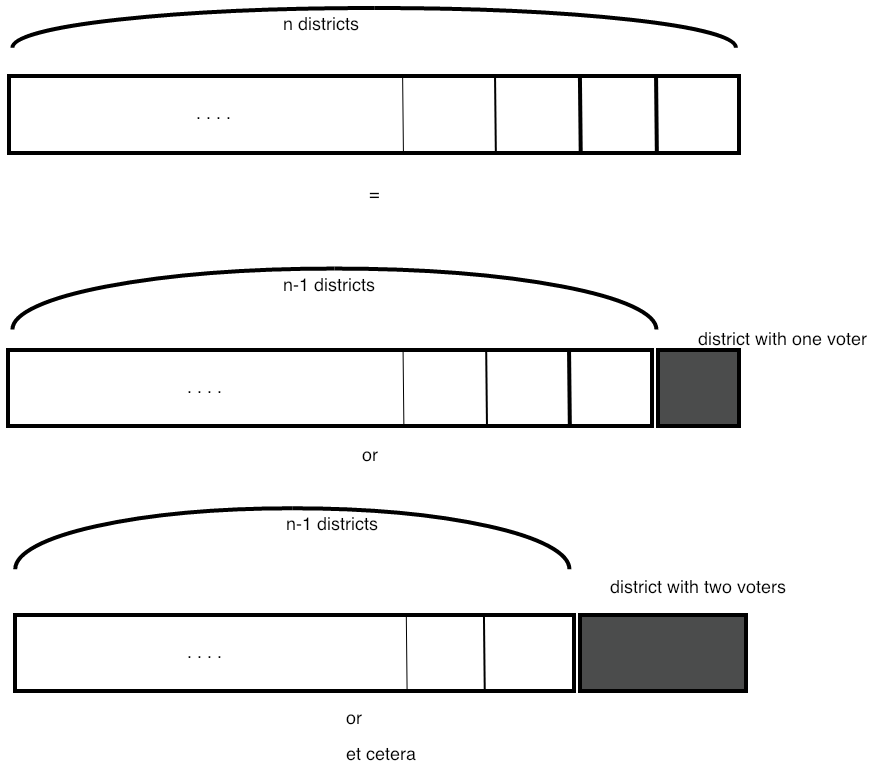
\includegraphics[scale=.4]{recursize-district}
  \caption{Multiple ways of splitting a population}
  \label{fig:recur-district}
\end{figure}

Now we need a method for districting a population:
\begin{lstlisting}
Districting Population::minority_rules( int ndistricts );
\end{lstlisting}
Rather than generating all possible partitions of the population, we
take an incremental approach (this is related to the solution strategy
called \indextermsub{dynamic}{programming}):
\begin{itemize}
\item The basic question is to divide a population optimally over $n$
  districts;
\item We do this recursively by first solving a division of a subpopulation over $n-1$
  districts,
  \item and extending that with the remaining population as one district.
\end{itemize}
This means that you need to consider all the ways of having the
`remaining' population into one district, and that means that you will
have a loop over all ways of splitting the population, outside of your
recursion; see figure~\textbookref{fig:recur-district}.
\begin{itemize}
\item For all $p=0,\ldots n-1$ considering splitting the state into
  $0,\ldots,p-1$ and $p,\ldots,n-1$.
\item Use the best districting of the first group, and make the last
  group into a single district.
\item Keep the districting that gives the strongest minority rule,
  over all values of~$p$.
\end{itemize}

You can now realize the above simple example:
\begin{verbatim}
AAABB => AAA|B|B
\end{verbatim}

\begin{exercise}
  Implement the above scheme.
  %
  \answerwithoutput{district5}{gerry}{district5}

  Note: the range for $p$ given above is not quite correct: for instance,
  the initial part of the population needs to be big enough to
  accomodate $n-1$ voters.
\end{exercise}

\begin{exercise}
  Test multiple population sizes; how much majority can you give
  party~B while still giving party~A a majority.
\end{exercise}

\Level 0 {Efficiency: dynamic programming}

If you think about the algorithm you just implemented, you may notice
that the districtings of the initial parts get recomputed quite a bit.
A~strategy for optimizing for this is called \indexterm{memoization}.

\begin{exercise}
  Improve your implementation by storing and reusing results for the
  initial sub-populations.
\end{exercise}

In a way, we solved the program backward: we looked at making a
district out of the last so-many voters, and then recursively solving
a smaller problem for the first however-many voters. But in that
process, we decided what is the best way to assign districts to the
first 1~voter, first~2, first~3, et cetera. Actually, for more than
one voter, say five voters, we found the result on the best attainable
minority rule assigning these five voters to one, two, three, four
districts.

The process of computing the `best' districting forward, is known as
\indextermbus{dynamic}{programming}. The fundamental assumption here
is that you can use intermediate results and extend them, without
having to reconsider the earlier problems.

Consider for instance that you've considered districting ten voters over up to
five districts. Now the majority for eleven voters and five districts
is the minimum of
\begin{itemize}
\item ten voters and five districts, and the new voter is added to the
  last district; or
\item ten voters and four districts, and the new voter becomes a new district.
\end{itemize}

\begin{comment}
\begin{itemize}
\item If you know the results for districting ten voters:
  \begin{itemize}
  \item you know the overall district majority, and
  \item you know the majority in the last district
  \end{itemize}
\item then for eleven voters you can
  \begin{itemize}
  \item add the new voter to the previous district, and compute the
    new majorities, overall and in the last district, or
  \item turn the new voter into a new district, and compute the two majorities.
  \end{itemize}
\item You need to compute the implications of adding the new voter,
  once for each possible districting of ten voters. 
\end{itemize}
\end{comment}

\begin{exercise}
  Code a dynamic programming solution to the redistricting problem. 
\end{exercise}

\Level 0 {Extensions}

The project so far has several simplifying assumptions.
\begin{itemize}
\item Congressional districts need to be approximately the same
  size. Can you put a limit on the ratio between sizes? Can the
  minority still gain a majority?
\end{itemize}

\begin{exercise}
  The biggest assumption is of course that we considered a
  one-dimensional state. With two dimensions you have more degrees of
  freedom of shaping the districts. Implement a two-dimensional
  scheme; use a completely square state, where the census districts
  form a regular grid. Limit the shape of the congressional districts
  to be convex.
\end{exercise}

The \indexterm{efficiency gap} is a measure of how `fair' a
districting of a state is. 

\begin{exercise}
  Look up the definition of efficiency gap (and `wasted votes'), and
  implement it in your code.
\end{exercise}

\Level 0 {Ethics}

The activity of redistricting was intended to give people a fair representation.
In its degenerate form of Gerrymandering this concept of fairness is violated
because the explicit goal is to give the minority a majority of votes.
Explore ways that this unfairness can be undone.

In your explorations above, the only characteristic of a voter was their preference
for party A or~B. However, in practice voters can be considered part of communities.
The Voting Rights Act is concerned about `minority vote dilution'.
Can you show examples that a color-blind districting
would affect some communities negatively?
